% Importado desde: 2026-03-28_Derivacion_Grafeno_a_Dirac.tex
\chapter{Derivacion Pedagogica: --- De la red honeycomb de grafeno al Hamiltoniano de Dirac en \(2+1\)}
\label{ch:derivacion-grafeno-a-dirac}

\section{Objetivo}

La meta de este documento es derivar, de manera lenta y explicita, como la ecuacion efectiva de Dirac aparece en grafeno a partir de un modelo tight-binding de primeros vecinos sobre la red honeycomb. La idea es dejar un texto autocontenido, con figuras y cuentas intermedias, que sirva como base de estudio antes de pasar a una formulacion mas tecnica de materiales de Dirac y Weyl en tres dimensiones.

La cadena conceptual que vamos a recorrer es:
\[
\begin{aligned}
\text{red honeycomb}
&\longrightarrow
\text{Hamiltoniano tight-binding}
\longrightarrow
\text{matriz de Bloch } H(\vk)
\\
&\longrightarrow
\text{puntos } K,K'
\longrightarrow
\text{expansion lineal}
\longrightarrow
\text{Hamiltoniano de Dirac efectivo.}
\end{aligned}
\]

\section{Panorama general}

Grafeno tiene dos ingredientes estructurales esenciales:

\begin{enumerate}[leftmargin=*]
  \item la red no es una red de Bravais simple, sino una red de Bravais triangular con una base de dos atomos;
  \item esos dos atomos por celda unitaria definen dos subredes, tradicionalmente llamadas \(A\) y \(B\).
\end{enumerate}

Como el electron puede saltar entre primeros vecinos de \(A\) a \(B\), el Hamiltoniano natural tiene una estructura \(2\times 2\) en el espacio de subred. Esa estructura matricial es la semilla del pseudospin de grafeno y es la razon por la que las matrices de Pauli aparecen naturalmente en la teoria efectiva.

\section{La red honeycomb en espacio real}

\subsection{Subredes y vectores de primeros vecinos}

Tomamos una convencion sencilla para los tres vectores que conectan un sitio de la subred \(A\) con sus tres vecinos mas cercanos de la subred \(B\):
\begin{equation}
\vdelta_1 = a(0,-1),
\qquad
\vdelta_2 = a\left(\frac{\sqrt{3}}{2},\frac{1}{2}\right),
\qquad
\vdelta_3 = a\left(-\frac{\sqrt{3}}{2},\frac{1}{2}\right),
\label{eq:deltas}
\end{equation}
donde \(a\) es la distancia entre atomos vecinos.

Con esta eleccion, dos vectores primitivos de la red de Bravais triangular asociada a la subred \(A\) pueden tomarse como
\begin{equation}
\va_1 = \vdelta_2 - \vdelta_3 = a(\sqrt{3},0),
\qquad
\va_2 = \vdelta_3 - \vdelta_1 = a\left(-\frac{\sqrt{3}}{2},\frac{3}{2}\right).
\label{eq:primitive-real}
\end{equation}

\begin{figure}[ht]
\centering
\begin{tikzpicture}[scale=1.45,>=Latex]
  \coordinate (A0) at (0,0);
  \coordinate (B1) at (0,-1);
  \coordinate (B2) at (0.866,0.5);
  \coordinate (B3) at (-0.866,0.5);
  \coordinate (Ar) at (1.732,0);
  \coordinate (Al) at (-1.732,0);
  \coordinate (Aul) at (-0.866,1.5);
  \coordinate (Aur) at (0.866,1.5);
  \coordinate (Adl) at (-0.866,-1.5);
  \coordinate (Adr) at (0.866,-1.5);
  \coordinate (Br1) at (1.732,1);
  \coordinate (Br2) at (1.732,-1);
  \coordinate (Bl1) at (-1.732,1);
  \coordinate (Bl2) at (-1.732,-1);

  \foreach \p/\q in {
    A0/B1,A0/B2,A0/B3,
    Ar/B2,Ar/Br1,Ar/Br2,
    Al/B3,Al/Bl1,Al/Bl2,
    Aul/B2,Aul/B3,Aul/Bl1,
    Aur/B2,Aur/B3,Aur/Br1,
    Adl/B1,Adl/B3,Adl/Bl2,
    Adr/B1,Adr/B2,Adr/Br2}
    \draw[gray!70,line width=0.8pt] (\p) -- (\q);

  \foreach \p in {A0,Ar,Al,Aul,Aur,Adl,Adr}
    \fill[blue!70] (\p) circle (2.2pt);
  \foreach \p in {B1,B2,B3,Br1,Br2,Bl1,Bl2}
    \fill[orange!85!black] (\p) circle (2.2pt);

  \node[above left=1pt of A0] {$A$};
  \node[right=1pt of B2] {$B$};

  \draw[->,very thick,red!75!black] (A0) -- (B1) node[midway,right] {$\vdelta_1$};
  \draw[->,very thick,red!75!black] (A0) -- (B2) node[midway,above right] {$\vdelta_2$};
  \draw[->,very thick,red!75!black] (A0) -- (B3) node[midway,above left] {$\vdelta_3$};

  \draw[->,thick,blue!80!black] (A0) -- (Ar) node[midway,below] {$\va_1$};
  \draw[->,thick,blue!80!black] (A0) -- (Aul) node[midway,left] {$\va_2$};

  \node[below left] at (-2.15,-1.85) {\footnotesize subred $A$};
  \fill[blue!70] (-2.48,-1.83) circle (2pt);
  \node[below left] at (-2.15,-2.12) {\footnotesize subred $B$};
  \fill[orange!85!black] (-2.48,-2.10) circle (2pt);
\end{tikzpicture}
\caption{Patch local de la red honeycomb de grafeno. Los sitios azules forman la subred \(A\) y los naranjas la subred \(B\). Los vectores \(\vdelta_i\) conectan primeros vecinos \(A\to B\), mientras que \(\va_1,\va_2\) generan la red de Bravais subyacente.}
\label{fig:honeycomb}
\end{figure}

\subsection{Por que aparecen dos componentes en la funcion de onda}

Como hay dos sitios distintos por celda, la amplitud de la funcion de onda debe llevar dos componentes:
\begin{equation}
\Psi(\vR) =
\begin{pmatrix}
\psi_A(\vR)\\[4pt]
\psi_B(\vR)
\end{pmatrix}.
\end{equation}

Esta estructura de dos componentes no es el espin real del electron. Es un grado de libertad de subred, y por eso se le llama \textit{pseudospin}. Mas adelante las matrices de Pauli \(\sigma_x,\sigma_y,\sigma_z\) actuaran sobre este espacio \(A/B\).

\section{Hamiltoniano tight-binding}

\subsection{El modelo minimo}

En el modelo mas simple retenemos solo saltos entre primeros vecinos y un unico parametro de hopping \(t\). El Hamiltoniano es
\begin{equation}
H = -t \sum_{\vR}\sum_{j=1}^3
\left(
a_{\vR}^\dagger b_{\vR+\vdelta_j}
+ b_{\vR+\vdelta_j}^\dagger a_{\vR}
\right),
\label{eq:tb-real}
\end{equation}
donde:

\begin{enumerate}[leftmargin=*]
  \item \(a_{\vR}^\dagger\) crea un electron en la subred \(A\) de la celda \(\vR\);
  \item \(b_{\vR+\vdelta_j}^\dagger\) crea un electron en uno de los tres vecinos \(B\);
  \item el signo menos es la convencion usual del tight-binding para que la banda de conduccion y valencia queden simetricas alrededor de cero.
\end{enumerate}

\subsection{Lectura fisica de la ecuacion}

La expresion \eqref{eq:tb-real} dice algo muy concreto: un electron sentado en \(A\) puede saltar a cualquiera de sus tres vecinos \(B\), y viceversa. Toda la estructura no trivial de grafeno aparece porque esos tres caminos interfieren entre si cuando pasamos al espacio de momentos.

\section{Paso al espacio recíproco}

\subsection{Transformadas de Fourier}

Definimos
\begin{equation}
a_{\vR} = \frac{1}{\sqrt{N}}\sum_{\vk}\ee^{\ii \vk\cdot\vR} a_{\vk},
\qquad
b_{\vR+\vdelta_j} = \frac{1}{\sqrt{N}}\sum_{\vk}\ee^{\ii \vk\cdot(\vR+\vdelta_j)} b_{\vk},
\label{eq:fourier}
\end{equation}
con \(N\) el numero de celdas unitarias.

Sustituyendo \eqref{eq:fourier} en \eqref{eq:tb-real} se obtiene
\begin{align}
H
&=
-t \sum_{\vR}\sum_{j=1}^3
\left[
\left(\frac{1}{\sqrt{N}}\sum_{\vk}\ee^{-\ii \vk\cdot\vR}a_{\vk}^\dagger\right)
\left(\frac{1}{\sqrt{N}}\sum_{\vk'}\ee^{\ii \vk'\cdot(\vR+\vdelta_j)}b_{\vk'}\right)
+ \text{h.c.}
\right]
\nonumber\\[4pt]
&=
-\frac{t}{N}\sum_{\vR}\sum_{j=1}^3\sum_{\vk,\vk'}
\ee^{\ii(\vk'-\vk)\cdot\vR}\,
\ee^{\ii \vk'\cdot\vdelta_j}\,
a_{\vk}^\dagger b_{\vk'}
+ \text{h.c.}
\label{eq:before-orthogonality}
\end{align}

Ahora usamos la identidad de ortogonalidad
\begin{equation}
\sum_{\vR}\ee^{\ii(\vk'-\vk)\cdot\vR}=N\,\delta_{\vk,\vk'}.
\end{equation}

Con esto, la suma en \(\vR\) fuerza \(\vk'=\vk\), y queda
\begin{equation}
H=
-t\sum_{\vk}\sum_{j=1}^3
\left(
\ee^{\ii \vk\cdot\vdelta_j} a_{\vk}^\dagger b_{\vk}
+ \ee^{-\ii \vk\cdot\vdelta_j} b_{\vk}^\dagger a_{\vk}
\right).
\label{eq:hk-sum}
\end{equation}

\subsection{La matriz de Bloch}

Introducimos la funcion estructural
\begin{equation}
f(\vk)=\sum_{j=1}^3 \ee^{\ii \vk\cdot\vdelta_j}.
\label{eq:fk}
\end{equation}

Entonces \eqref{eq:hk-sum} se escribe como
\begin{equation}
H = \sum_{\vk}
\begin{pmatrix}
a_{\vk}^\dagger & b_{\vk}^\dagger
\end{pmatrix}
\begin{pmatrix}
0 & -t f(\vk)\\
-t f^*(\vk) & 0
\end{pmatrix}
\begin{pmatrix}
a_{\vk}\\
b_{\vk}
\end{pmatrix}.
\label{eq:bloch-matrix}
\end{equation}

Asi, el Hamiltoniano de una sola particula es
\begin{equation}
H(\vk)=
\begin{pmatrix}
0 & -t f(\vk)\\
-t f^*(\vk) & 0
\end{pmatrix}.
\label{eq:Hk}
\end{equation}

\section{Bandas de energia}

\subsection{Calculo de autovalores}

Los autovalores se obtienen de
\begin{equation}
\det\!\big(H(\vk)-E I\big)=0.
\end{equation}

Como
\begin{equation}
\det
\begin{pmatrix}
-E & -t f(\vk)\\
-t f^*(\vk) & -E
\end{pmatrix}
= E^2 - t^2 |f(\vk)|^2,
\end{equation}
resulta
\begin{equation}
E_\pm(\vk)=\pm t |f(\vk)|.
\label{eq:dispersion-general}
\end{equation}

Esto ya muestra dos cosas fundamentales:

\begin{enumerate}[leftmargin=*]
  \item hay dos bandas, una de conduccion y una de valencia;
  \item el contacto entre ellas ocurre cuando \(f(\vk)=0\).
\end{enumerate}

\subsection{Forma explicita de f(k)}

Usando los vectores \eqref{eq:deltas},
\begin{align}
f(\vk)
&=
\ee^{-\ii a k_y}
+ \ee^{\ii\left(\frac{\sqrt{3}}{2}a k_x+\frac{1}{2}a k_y\right)}
+ \ee^{\ii\left(-\frac{\sqrt{3}}{2}a k_x+\frac{1}{2}a k_y\right)}
\nonumber\\[4pt]
&=
\ee^{-\ii a k_y}
+ 2\,\ee^{\ii a k_y/2}\cos\!\left(\frac{\sqrt{3}}{2}a k_x\right).
\label{eq:fk-explicit}
\end{align}

Al tomar el modulo al cuadrado se obtiene
\begin{equation}
|f(\vk)|^2
=
1
+4\cos^2\!\left(\frac{\sqrt{3}}{2}a k_x\right)
+4\cos\!\left(\frac{\sqrt{3}}{2}a k_x\right)\cos\!\left(\frac{3}{2}a k_y\right).
\label{eq:fk-mod}
\end{equation}

Por tanto,
\begin{equation}
E_\pm(\vk)=
\pm t
\sqrt{
1
+4\cos^2\!\left(\frac{\sqrt{3}}{2}a k_x\right)
+4\cos\!\left(\frac{\sqrt{3}}{2}a k_x\right)\cos\!\left(\frac{3}{2}a k_y\right)
}.
\label{eq:graphene-dispersion}
\end{equation}

\section{La zona de Brillouin y los puntos de Dirac}

\subsection{Donde se tocan las bandas}

Las bandas se tocan cuando \(f(\vk)=0\). Una solucion especialmente importante es
\begin{equation}
\vK=\left(\frac{4\pi}{3\sqrt{3}a},0\right),
\qquad
\vK'=\left(-\frac{4\pi}{3\sqrt{3}a},0\right).
\label{eq:KKp}
\end{equation}

Verificacion rapida en \(\vK\):
\begin{equation}
f(\vK)
=
1+\ee^{\ii 2\pi/3}+\ee^{-\ii 2\pi/3}
=1+2\cos(2\pi/3)=0.
\end{equation}

La misma cancelacion ocurre en \(\vK'\). Estos son dos puntos no equivalentes de la primera zona de Brillouin y son justamente los puntos de Dirac.

\begin{figure}[ht]
\centering
\begin{tikzpicture}[scale=1.2,>=Latex]
  \def\R{2.3}
  \foreach \ang in {0,60,...,300}
    \coordinate (P\ang) at (\ang:\R);

  \draw[thick] (P0)--(P60)--(P120)--(P180)--(P240)--(P300)--cycle;
  \draw[->] (-2.8,0) -- (2.8,0) node[right] {$k_x$};
  \draw[->] (0,-2.5) -- (0,2.7) node[above] {$k_y$};

  \fill (0,0) circle (2pt);
  \node[below left] at (0,0) {$\Gamma$};

  \coordinate (K) at (1.53,0);
  \coordinate (Kp) at (-1.53,0);
  \fill[red!80!black] (K) circle (2.2pt);
  \fill[red!80!black] (Kp) circle (2.2pt);
  \node[below] at (K) {$K$};
  \node[below] at (Kp) {$K'$};

  \draw[blue!80!black,thick,->] (K) -- ++(0.55,0.45) node[above right] {$\vq$};
  \draw[blue!80!black,thick,->] (Kp) -- ++(-0.55,0.45) node[above left] {$\vq$};

  \draw[gray!60,dashed] (K) circle (0.38);
  \draw[gray!60,dashed] (Kp) circle (0.38);

  \node[align=center] at (0,2.15) {\footnotesize Primera zona de Brillouin\\ \footnotesize y regiones de expansion de baja energia};
\end{tikzpicture}
\caption{Primera zona de Brillouin esquematica para grafeno. Los puntos \(K\) y \(K'\) son los puntos no equivalentes donde se anulan simultaneamente las bandas y alrededor de los cuales se hace la expansion lineal \(\vk=\vK+\vq\) o \(\vk=\vK'+\vq\).}
\label{fig:bz}
\end{figure}

\subsection{Significado fisico}

La anulacion de \(f(\vk)\) no es accidental. Es una interferencia destructiva exacta entre los tres caminos de hopping desde un sitio de la subred \(A\) hacia los tres vecinos \(B\). Esa cancelacion obliga a que las bandas se toquen sin abrir gap en los puntos \(K\) y \(K'\).

\section{Expansion alrededor de K}

\subsection{Paso algebraico principal}

Escribimos
\begin{equation}
\vk=\vK+\vq,
\qquad |\vq| \ll |\vK|.
\end{equation}

Entonces
\begin{align}
f(\vK+\vq)
&=
\sum_{j=1}^3 \ee^{\ii (\vK+\vq)\cdot\vdelta_j}
=
\sum_{j=1}^3 \ee^{\ii \vK\cdot\vdelta_j}\ee^{\ii \vq\cdot\vdelta_j}.
\end{align}

Como \(|\vq\cdot\vdelta_j|\ll 1\), hacemos expansion a primer orden:
\begin{equation}
\ee^{\ii \vq\cdot\vdelta_j}\approx 1+\ii \vq\cdot\vdelta_j.
\end{equation}

Luego
\begin{equation}
f(\vK+\vq)\approx
\sum_{j=1}^3 \ee^{\ii \vK\cdot\vdelta_j}
+ \ii \sum_{j=1}^3 \ee^{\ii \vK\cdot\vdelta_j} \vq\cdot\vdelta_j.
\label{eq:f-expand-general}
\end{equation}

El primer termino se anula porque \(f(\vK)=0\). Por tanto
\begin{equation}
f(\vK+\vq)\approx
\ii \sum_{j=1}^3 \ee^{\ii \vK\cdot\vdelta_j} \vq\cdot\vdelta_j.
\label{eq:linear-term-only}
\end{equation}

\subsection{Cuenta explicita}

Para nuestra convencion,
\begin{equation}
\ee^{\ii \vK\cdot\vdelta_1}=1,
\qquad
\ee^{\ii \vK\cdot\vdelta_2}=\ee^{\ii 2\pi/3},
\qquad
\ee^{\ii \vK\cdot\vdelta_3}=\ee^{-\ii 2\pi/3}.
\end{equation}

Ademas,
\begin{align}
\vq\cdot\vdelta_1 &= -a q_y,
\nonumber\\
\vq\cdot\vdelta_2 &= a\left(\frac{\sqrt{3}}{2}q_x+\frac{1}{2}q_y\right),
\nonumber\\
\vq\cdot\vdelta_3 &= a\left(-\frac{\sqrt{3}}{2}q_x+\frac{1}{2}q_y\right).
\end{align}

Sustituyendo en \eqref{eq:linear-term-only},
\begin{align}
f(\vK+\vq)
&\approx
\ii \Bigg[
(-a q_y)
+ \ee^{\ii 2\pi/3}a\left(\frac{\sqrt{3}}{2}q_x+\frac{1}{2}q_y\right)
+ \ee^{-\ii 2\pi/3}a\left(-\frac{\sqrt{3}}{2}q_x+\frac{1}{2}q_y\right)
\Bigg].
\end{align}

Agrupamos \(q_x\) y \(q_y\) por separado:
\begin{align}
f(\vK+\vq)
&\approx
\ii a
\left[
\frac{\sqrt{3}}{2}\left(\ee^{\ii 2\pi/3}-\ee^{-\ii 2\pi/3}\right)q_x
+
\left(
-1+\frac{1}{2}\ee^{\ii 2\pi/3}+\frac{1}{2}\ee^{-\ii 2\pi/3}
\right)q_y
\right].
\end{align}

Usamos
\begin{equation}
\ee^{\ii 2\pi/3}-\ee^{-\ii 2\pi/3}=2\ii \sin(2\pi/3)=\ii\sqrt{3},
\end{equation}
y
\begin{equation}
\ee^{\ii 2\pi/3}+\ee^{-\ii 2\pi/3}=2\cos(2\pi/3)=-1.
\end{equation}

Entonces
\begin{align}
f(\vK+\vq)
&\approx
\ii a
\left[
\frac{\sqrt{3}}{2}(\ii\sqrt{3})q_x
+\left(-1-\frac{1}{2}\right)q_y
\right]
\nonumber\\[4pt]
&=
\ii a
\left[
\frac{3\ii}{2}q_x - \frac{3}{2}q_y
\right]
\nonumber\\[4pt]
&=
-\frac{3a}{2}(q_x+\ii q_y).
\label{eq:fK-final}
\end{align}

\subsection{Hamiltoniano efectivo cerca de K}

Insertando \eqref{eq:fK-final} en \eqref{eq:Hk},
\begin{equation}
H_K(\vq)
\approx
\frac{3at}{2}
\begin{pmatrix}
0 & q_x+\ii q_y\\
q_x-\ii q_y & 0
\end{pmatrix}.
\end{equation}

Definimos la velocidad de Fermi
\begin{equation}
v_F=\frac{3at}{2\hbar}.
\label{eq:vf}
\end{equation}

Entonces
\begin{equation}
H_K(\vq)
=
\hbar v_F
\begin{pmatrix}
0 & q_x+\ii q_y\\
q_x-\ii q_y & 0
\end{pmatrix}.
\label{eq:HK-matrix}
\end{equation}

En terminos de matrices de Pauli,
\begin{equation}
H_K(\vq)=\hbar v_F\,(q_x \sigma_x - q_y \sigma_y).
\label{eq:HK-pauli}
\end{equation}

Con una simple redefinicion unitaria de la base de subred, esta forma es equivalente a la version mas difundida
\begin{equation}
H_K(\vq)\sim \hbar v_F\,(q_x \sigma_x + q_y \sigma_y).
\label{eq:HK-standard}
\end{equation}

El punto importante no es el signo de una convencion de base, sino que el Hamiltoniano es lineal en \(\vq\) y tiene estructura exacta de Dirac sin masa en \(2+1\).

\section{Expansion alrededor de K'}

Ahora escribimos
\begin{equation}
\vk=\vK'+\vq,
\qquad
\vK'=-\vK.
\end{equation}

Repitiendo la expansion se obtiene
\begin{equation}
f(\vK'+\vq)\approx \frac{3a}{2}(q_x-\ii q_y).
\label{eq:fKp-final}
\end{equation}

Por tanto,
\begin{equation}
H_{K'}(\vq)
\approx
-\hbar v_F
\begin{pmatrix}
0 & q_x-\ii q_y\\
q_x+\ii q_y & 0
\end{pmatrix}.
\label{eq:HKp-matrix}
\end{equation}

De nuevo, dependiendo de la convencion de base, esto suele escribirse en forma compacta como
\begin{equation}
H_\tau(\vq)=\hbar v_F(\tau q_x \sigma_x + q_y \sigma_y),
\qquad \tau=\pm 1,
\label{eq:valley-compact}
\end{equation}
donde \(\tau=+1\) corresponde a \(K\) y \(\tau=-1\) a \(K'\).

\section{La dispersion lineal y el cono de Dirac}

\subsection{Autovalores de la teoria efectiva}

Para cualquiera de las dos valles, el Hamiltoniano efectivo tiene autovalores
\begin{equation}
E_\pm(\vq)=\pm \hbar v_F |\vq|.
\label{eq:dirac-dispersion}
\end{equation}

Esto es una dispersion lineal, no cuadratica. Cerca del punto de contacto, las bandas forman un cono superior y otro inferior: el famoso cono de Dirac.

\begin{figure}[ht]
\centering
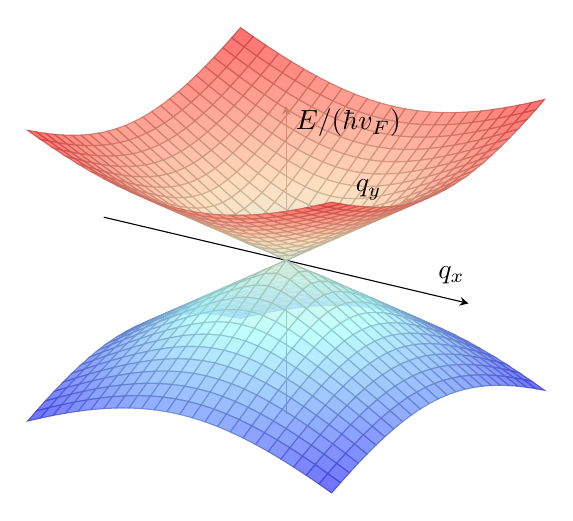
\begin{tikzpicture}
\begin{axis}[
  width=0.78\textwidth,
  view={35}{26},
  axis lines=center,
  xlabel={$q_x$},
  ylabel={$q_y$},
  zlabel={$E/(\hbar v_F)$},
  xmin=-1.2,xmax=1.2,
  ymin=-1.2,ymax=1.2,
  zmin=-1.5,zmax=1.5,
  ticks=none,
  colormap={mycmap}{
    color=(blue!70)
    color=(cyan!30)
    color=(orange!30)
    color=(red!70)
  },
  samples=25,
  domain=-1:1,
  y domain=-1:1
]
\addplot3[surf,opacity=0.82] {sqrt(x^2+y^2)};
\addplot3[surf,opacity=0.82] {-sqrt(x^2+y^2)};
\end{axis}
\end{tikzpicture}
\caption{Dispersion efectiva cerca de un punto de Dirac. La energia es lineal en \(|\vq|\), de modo que las bandas de conduccion y valencia forman un doble cono que se toca en \(E=0\).}
\label{fig:cone}
\end{figure}

\subsection{Interpretacion}

La ecuacion \eqref{eq:dirac-dispersion} es la firma de fermiones relativistas efectivos sin masa. La velocidad de la luz \(c\) de la teoria relativista es reemplazada aqui por la velocidad de Fermi \(v_F\), y las matrices de Pauli actuan sobre el pseudospin de subred en lugar del espin real.

\section{Como se lee esto como ecuacion de Dirac}

\subsection{Del Hamiltoniano a la ecuacion de movimiento}

La ecuacion de Schrodinger efectiva es
\begin{equation}
\ii \hbar \,\partial_t \Psi = H_\tau \Psi.
\end{equation}

Usando \eqref{eq:valley-compact},
\begin{equation}
\ii \hbar \,\partial_t \Psi
=
\hbar v_F(\tau q_x \sigma_x + q_y \sigma_y)\Psi.
\end{equation}

Al pasar a espacio real, \(q_x\to -\ii\partial_x\) y \(q_y\to -\ii\partial_y\), de modo que
\begin{equation}
\ii \partial_t \Psi
=
-\ii v_F(\tau \sigma_x \partial_x + \sigma_y \partial_y)\Psi.
\label{eq:dirac-real-space}
\end{equation}

Esta es exactamente una ecuacion de Dirac sin masa en \(2+1\), escrita en una representacion adaptada al problema de grafeno.

\subsection{Que representa cada simbolo}

\begin{center}
\begin{tabular}{p{0.28\textwidth}p{0.58\textwidth}}
\toprule
\textbf{Objeto} & \textbf{Interpretacion en grafeno} \\
\midrule
\(\Psi\) & espinor de dos componentes en subred \(A/B\) \\
\(\sigma_x,\sigma_y,\sigma_z\) & matrices de Pauli sobre el pseudospin \\
\(\tau=\pm 1\) & indice de valle, asociado a \(K\) y \(K'\) \\
\(v_F\) & velocidad de Fermi efectiva \\
\(E=\pm \hbar v_F |\vq|\) & dispersion lineal tipo fermion sin masa \\
\bottomrule
\end{tabular}
\end{center}

\section{Resumen paso por paso}

\begin{enumerate}[leftmargin=*]
  \item La red honeycomb se descompone en dos subredes, \(A\) y \(B\).
  \item Eso obliga a usar una funcion de onda de dos componentes.
  \item El modelo tight-binding de primeros vecinos produce una matriz \(2\times 2\) en el espacio de subred.
  \item En espacio recíproco, toda la informacion geometrica queda contenida en \(f(\vk)=\sum_j \ee^{\ii \vk\cdot\vdelta_j}\).
  \item Las bandas se tocan cuando \(f(\vk)=0\), lo que ocurre en \(K\) y \(K'\).
  \item Al expandir \(\vk=\vK+\vq\) o \(\vk=\vK'+\vq\), el Hamiltoniano se vuelve lineal en \(\vq\).
  \item Esa expansion lineal es el Hamiltoniano de Dirac efectivo de grafeno.
\end{enumerate}

\begin{figure}[ht]
\centering
\begin{tikzpicture}[
  node distance=8mm and 10mm,
  every node/.style={font=\small},
  box/.style={draw,rounded corners,thick,align=center,minimum width=3.1cm,minimum height=0.95cm,fill=blue!6},
  arr/.style={-{Latex[length=3mm]},thick}
]
  \node[box] (r1) {Red honeycomb\\ dos subredes \(A/B\)};
  \node[box, right=of r1] (r2) {Hamiltoniano\\ tight-binding};
  \node[box, right=of r2] (r3) {Matriz de Bloch\\ \(H(\vk)\)};
  \node[box, below=of r2] (r4) {Ceros de \(f(\vk)\)\\ puntos \(K\) y \(K'\)};
  \node[box, left=of r4] (r5) {Expansion\\ \(\vk=\vK+\vq\)};
  \node[box, right=of r4] (r6) {Hamiltoniano lineal\\ \(\hbar v_F\,\bm{\sigma}\cdot\vq\)};

  \draw[arr] (r1) -- (r2);
  \draw[arr] (r2) -- (r3);
  \draw[arr] (r3) -- (r4);
  \draw[arr] (r4) -- (r5);
  \draw[arr] (r4) -- (r6);
\end{tikzpicture}
\caption{Mapa conceptual de la derivacion.}
\label{fig:flow}
\end{figure}

\section{Que dejamos listo para el siguiente paso}

Con esta derivacion ya quedan establecidas las piezas que hacen falta para avanzar luego hacia materiales de Dirac y Weyl:

\begin{enumerate}[leftmargin=*]
  \item el origen del pseudospin;
  \item la emergencia de una estructura tipo Dirac a baja energia;
  \item el papel de los valles \(K\) y \(K'\);
  \item la relacion entre simetria de red, linealidad del espectro y fermiones efectivos sin masa.
\end{enumerate}

El siguiente paso natural sera agregar perturbaciones controladas: masa, strain, campos externos o terminos spin-orbita. Esas deformaciones son las que permiten pasar de la fisica minima de grafeno a modelos mas cercanos a materiales de Dirac y Weyl.

\section{Observacion sobre convenciones}

En la literatura cambian con frecuencia:

\begin{enumerate}[leftmargin=*]
  \item la orientacion de los ejes;
  \item la definicion precisa de los vectores \(\vdelta_i\);
  \item el orden de la base \((A,B)\);
  \item la forma final del Hamiltoniano en \(K\) y \(K'\).
\end{enumerate}

Por eso pueden aparecer signos distintos delante de \(\sigma_x\) o \(\sigma_y\). Eso no cambia la fisica esencial. Lo que permanece invariante es:

\begin{enumerate}[leftmargin=*]
  \item la linealidad en \(\vq\);
  \item la estructura de dos componentes;
  \item la dispersion \(E=\pm \hbar v_F |\vq|\);
  \item la interpretacion de baja energia como fermiones de Dirac efectivos.
\end{enumerate}
